%% Included in decks: slidemage-manual
%%

% SlideMage manual, chapter "Working in SlideMage": the slide editor, on the
% standardframe demo slide (tools/manual/make_screenshots.py).
\begin{standardframe}{The slide editor}
	{\setlength{\fboxsep}{0pt}\fcolorbox{c_primary_gray}{white}{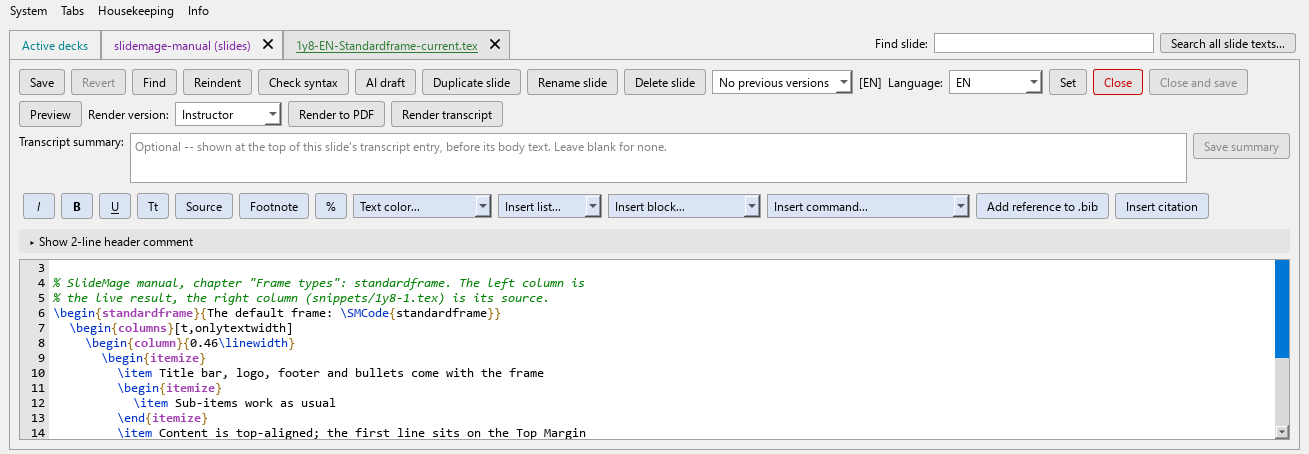
\includegraphics[width=0.66\linewidth]{media/screenshot-slidemage-slide-editor.png}}}\par\medskip
	\begin{columns}[t,onlytextwidth]
		\begin{column}{0.48\linewidth}
			\shrinklists{1}
			\begin{itemize}
				\item \emph{Render to PDF} compiles what is in the editor, saved or not; \emph{Preview} shows the last compile
				\item \emph{Save} with a version choice; find and replace, reindent, citations
			\end{itemize}
		\end{column}
		\begin{column}{0.48\linewidth}
			\shrinklists{1}
			\begin{itemize}
				\item Duplicate, rename, delete the slide; its language; its transcript summary
				\item With a local AI model: \emph{Check syntax}, \emph{AI draft} -- shown as a diff, applied only when you accept
			\end{itemize}
		\end{column}
	\end{columns}
\end{standardframe}
